\documentclass[10pt]{beamer}
\usepackage{physics}
\usepackage{amsfonts}
\usepackage{amsmath}
\usepackage{graphicx}
\graphicspath{{../images/}}
\usepackage[utf8]{inputenc}
\usetheme{Warsaw}
\usepackage[style=verbose]{biblatex}
\addbibresource{../References.bib}
\usepackage[justification=centering]{caption}
\captionsetup[figure]{labelformat=empty}
\useoutertheme{infolines}
\setbeamertemplate{navigation symbols}{}
%\setbeamertemplate{headline}{}
\usecolortheme{default}
\setbeamerfont{subsection in toc}{size=\small}
\setbeamerfont{footnote}{size=\tiny}
\expandafter\def\expandafter\insertshorttitle\expandafter{%
  \insertshorttitle\hfill%
  \insertframenumber\,/\,\inserttotalframenumber}
\title[E213 : Analysis of Decays of heavy vector boson $\rm Z^{0}$] %optional
{E213 : Analysis of Decays of heavy vector boson $\rm Z^{0}$}
\author[Sakthivasan, Jena] % (optional)
{Group P20: Ajay Shanmuga Sakthivasan \& Mrunmoy Jena\\
Supervisor: Martin Angelsmark}


\date{\today}

\begin{document}
\begin{frame}
    \titlepage 
\end{frame}

\begin{frame}
    \frametitle{Outline}
    \tableofcontents
\end{frame}

\section{Introduction}
\begin{frame}
\frametitle{Introduction}
\begin{itemize}
\item Goal: to understand how data from a particle accelerator is analysed and to deduce different properties of the $Z^0$ boson
\item Important physical quantities: $Z^0$ mass and decay width 
\item Data collected from the OPAL (Omni-Purpose Apparatus at LEP) detector
\item Part I: Carried out event display analysis on smaller datasets to understand how to separate out different $Z^0$ decay channels
\item Part II: Cuts (constraints) imposed on the data are refined and statistical analysis done on larger real world data $\rightarrow$ deduce physical quantities
\end{itemize}
\end{frame}

\section{Prerequisite Knowledge}
\subsection{Standard Model}
\begin{frame}
\frametitle{Standard Model}
\begin{minipage}{0.5\textwidth}
\begin{itemize}
\item Standard Model: provides the most fundamental description of nature by incorporating the elementary particles and their interactions
\item Two families: fermions (half integer spins), and bosons (integer spins)
\begin{itemize}
\item EM interactions $\rightarrow$ photon ($\gamma$)
\item Strong force $\rightarrow$ gluons (g) 
\item Weak force $\rightarrow$ $W^{\pm}, Z^{0}$ 
\item Gravity $\rightarrow$ graviton (hypothesized; not included in SM)
\end{itemize}
\end{itemize}
\end{minipage}\hspace{2em}
\begin{minipage}{0.35\textwidth}
      \begin{figure}
      \centering
        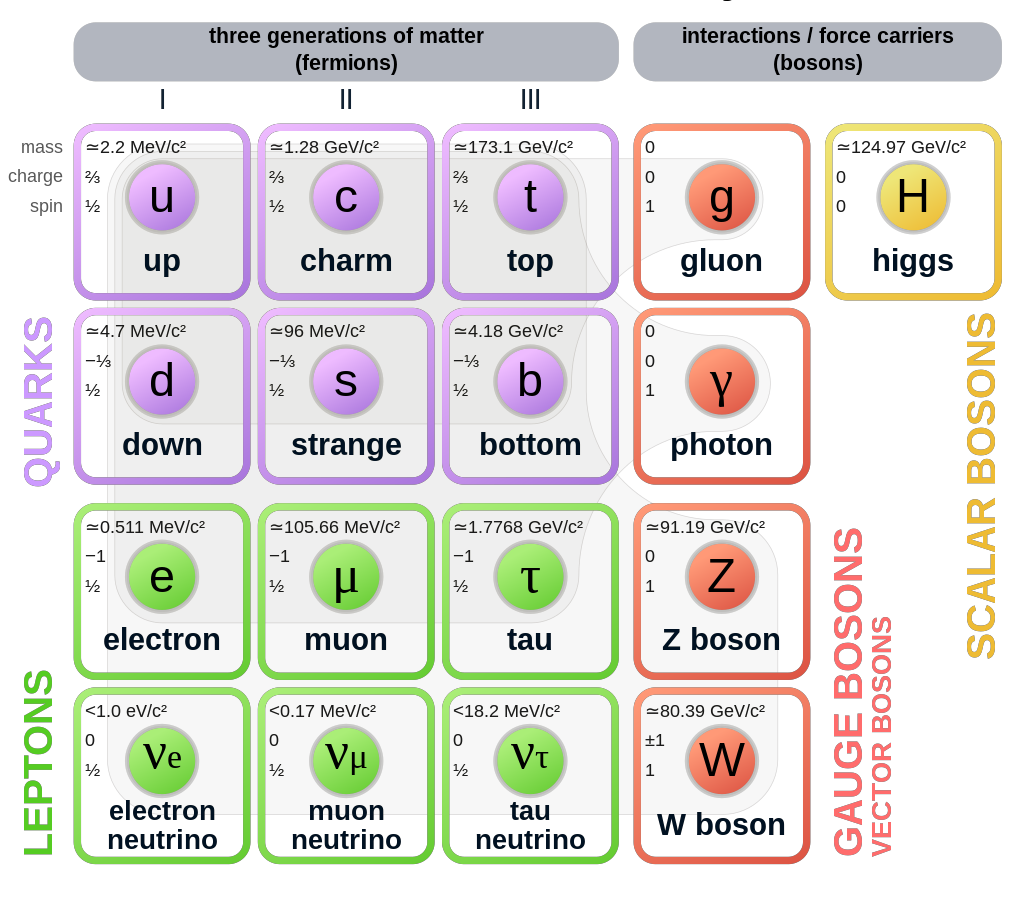
\includegraphics[height=\textwidth]{Standard_Model_of_Elementary_Particles}
        \caption{Standard Model \footnotemark{}}
      \end{figure}
  \end{minipage}\hfill
  \footcitetext{stdmodel}
\end{frame}

\begin{frame}
\frametitle{Standard Model}
\begin{itemize}
\item Fermions: three generations of quarks and leptons
\begin{itemize}
\item Six flavours of quarks: up (u), down (d), charm (c), strange (s), top (t) and bottom (b)
\item Six flavours of leptons: electron ($e$), muon ($\mu$) and tau ($\tau$), and associated neutrinos ($\nu_{e}$, $\nu_{\mu}$ and $\nu_{\tau}$)
\end{itemize}
\item Composite particles: three quark combinations, called baryons ($qqq$/$\bar{q}\bar{q}\bar{q}$) or quark-antiquark pairs, called  mesons ($q\bar{q}$)
\item Mathematically, elementary particles $\rightarrow$ elements of representations of certain symmetry groups
\item Gauge fields coupling to these particles $\rightarrow$ consequence of invariance of corresponding Lagrangian under local phase transformations \footnotemark{}
\item Gauge symmetry that governs the Standard Model is given by: $$SU(3)_{\mathrm{Colour}}\times SU(2)_{\mathrm{Left\ chiral}}\times U(1)_{\mathrm{Y}(\mathrm{Weak \ hypercharge})}$$
\end{itemize}
\footcitetext{thomson_2013}
\end{frame}

\subsection{Electroweak Theory}
\begin{frame}
\frametitle{Electroweak Theory}
\begin{itemize}
\item Initially, EM and the theory of weak interactions formulated separately
\item At higher energies ($\sim$ 246 GeV \footnotemark{}), unified into single force $\rightarrow$ GSW electroweak model - 1960s
\item Impose local gauge invariance on $SU(2)_{L}$ symmetry group $\rightarrow$ three gauge fields: $W^{(1)},\ W^{(2)}$ and $W^{(3)}$
\item Physical $W^{+}$ and $W^{-}$ bosons found to be linear combinations: 
\begin{equation}
W^{\pm}_{\mu}=\dfrac{1}{\sqrt{2}}\left(W^{(1)}_{\mu}\mp \rm{i}W^{(2)}_{\mu}\right)
\end{equation}
\end{itemize}
\footcitetext{pdg-ew}
\end{frame}

\begin{frame}
\frametitle{Electroweak Theory}
\begin{itemize}
\item $W^{(3)}_{\mu}$ field (no physical interpretation ?)
\item Additional symmetry, the $U(1)_{Y}$ group is introduced
\item $B_{\mu}$ field arising from $U(1)_{Y}$ symmetry (no physical meaning ?)
\item Linear combinations of $W^{(3)}_{\mu}$ and $B_{\mu}$ fields $\rightarrow$ photon and the $Z^{0}$ boson:
\begin{equation}
\begin{pmatrix} 
A_{\mu} \\ 
Z_{\mu} 
\end{pmatrix}
= 
\begin{pmatrix}
\cos \theta_{W} & \sin \theta_{W} \\
-\sin \theta_{W} & \cos \theta_{W} 
\end{pmatrix}
\begin{pmatrix}
B_{\mu} \\
W^{(3)}_{\mu}
\end{pmatrix}
\end{equation}
$\theta_{W}$ : weak mixing/Weinberg angle
\end{itemize}
\end{frame}

\subsection{Physics Related to the $Z^{0}$ Resonance}
\subsubsection{Angular Dependence of $\gamma / Z^{0}$ Mediated Processes}
\begin{frame}
\frametitle{Angular Dependence of $\gamma / Z^{0}$ Mediated Processes}
\begin{minipage}{0.5\textwidth}
\begin{itemize}
\item $e^{+}e^{-}\rightarrow e^{+}e^{-}$: t-channel as well as s-channel component
\item $e^{+}e^{-}\rightarrow f\bar{f}$ ($f$ other than $e^{-}$): only s-channel
\end{itemize}
\end{minipage}\hspace{2em}
\begin{minipage}{0.35\textwidth}
      \begin{figure}
      \centering
        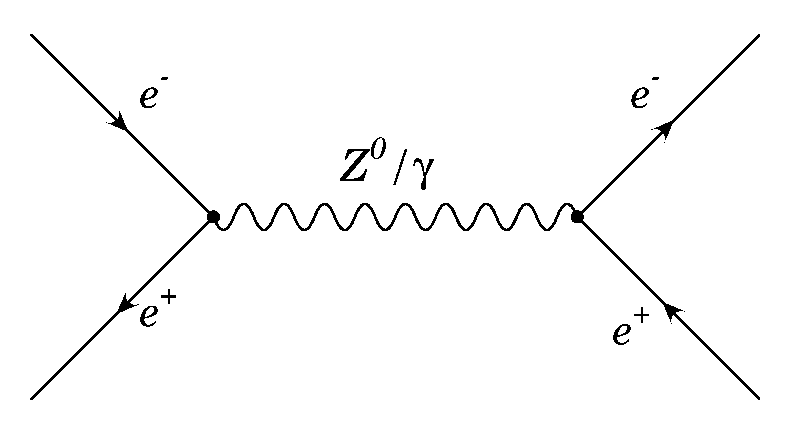
\includegraphics[width=\textwidth]{bhabha-s}
        \caption{$s$-channel Bhaba scattering}
      \end{figure}
      \begin{figure}
      \centering
        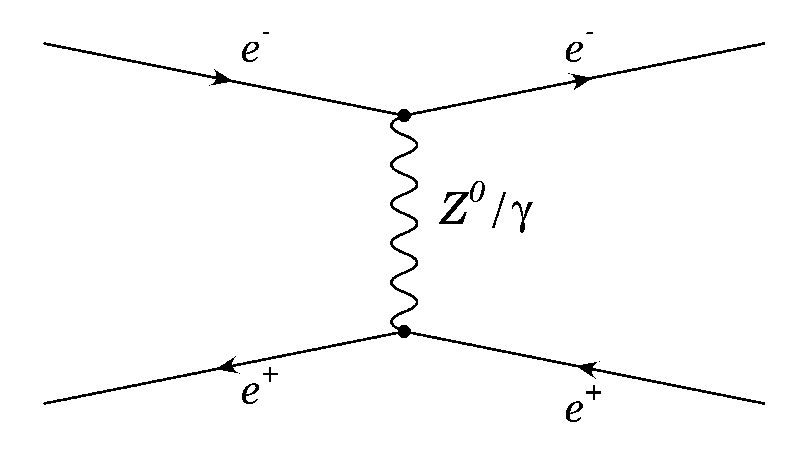
\includegraphics[width=\textwidth]{bhabha-t}
        \caption{$t$-channel Bhaba scattering}
      \end{figure}
  \end{minipage}\hfill
\end{frame}

\begin{frame}
\frametitle{Angular Dependence of $\gamma / Z^{0}$ Mediated Processes}
\begin{minipage}{0.5\textwidth}
\begin{itemize}
\item $s$ channel angular dependence: $\left(\dfrac{d\sigma}{d\Omega}\right)_{s}\propto (1+\cos^{2}\theta)$

Cross section has a major contribution at large angles (or small values of $\cos\theta$)
\item $t$ channel angular dependence: $\left(\dfrac{d\sigma}{d\Omega}\right)_{t}\propto (1-\cos\theta)^{-2}$
Cross section increases asymptotically at small angles (or large values of $\cos\theta$)\footnotemark{}
\item Essential step ! : Remove $t$-channel contribution while finding inherent forward backward asymmetry in $e^{+}e^{-}\rightarrow e^{+}e^{-}$ process
\end{itemize}
\end{minipage}\hspace{1em}
\begin{minipage}{0.45\textwidth}
\begin{figure}
\centering
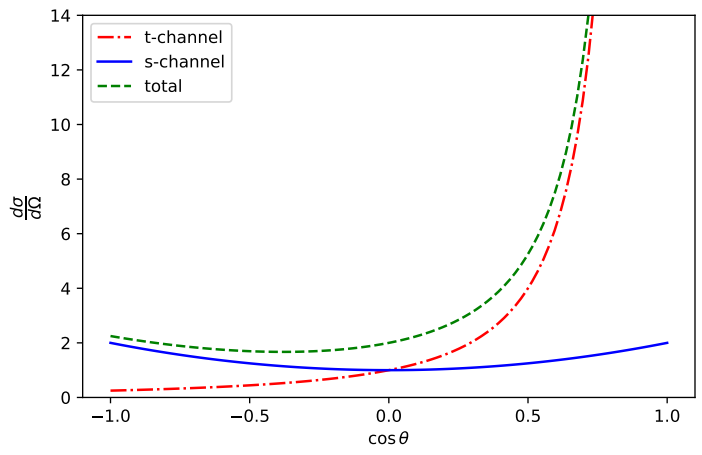
\includegraphics[width=\textwidth]{tangulardist}
\caption{$s$ and $t$-channel angular distribution}
\end{figure}
\end{minipage}\hfill
\footcitetext{UB}
\end{frame}

\subsubsection{Forward-Backward Asymmetry}
\begin{frame}
\frametitle{Forward-Backward Asymmetry}
\begin{itemize}
\item Consider $Z^{0}$ mediated $s$-channel process $e^{+}e^{-}\rightarrow f\bar{f}$
\item Angular dependence:
\vspace{0.5em}
$\left(\dfrac{d\sigma}{d\Omega}\right)_{s\ (Z^{0})}\propto a(1+\cos^{2}\theta) + 2b\cos\theta$
\item No. of fermions in forward dir., ($\theta>\pi /2$) $\neq$ no. of fermions in backward dir., ($\theta<\pi /2$)
\item Asymmetry term $b$: Due to unequal coupling of $Z^{0}$ to right handed and left handed fermions
\vspace{0.5em}
$b=\left[\left(g_{L}^{e}\right)^{2}-\left(g_{R}^{e}\right)^{2}\right]\left[\left(g_{L}^{f}\right)^{2}-\left(g_{R}^{f}\right)^{2}\right]$
\begin{itemize}
\item $g_{L}^{f}$: coupling of $Z^{0}$ to left handed fermions
\item $g_{R}^{f}$: coupling of $Z^{0}$ to right handed fermions
\end{itemize}
\end{itemize}
\end{frame}

\begin{frame}
\frametitle{Forward-Backward Asymmetry}
\begin{itemize}
\item FB asymmetry factor given as the ratio:
\vspace{0.5em}
$\mathcal{A}_{fb}=\dfrac{\sigma_{F}-\sigma_{B}}{\sigma_{F}+\sigma_{B}}=\dfrac{3b}{4a}$
\begin{itemize}
\item $\sigma_{F}, \sigma_{B}$: cross sections in forward and backward directions respectively
\end{itemize}
\item At $Z^{0}$  resonance, $\mathcal{A}_{fb}$ simplifies to \footnotemark{}:
\vspace{0.5em}
$\mathcal{A}_{fb}^{f}\approx 3\left(\dfrac{g_{V}^{f}}{g_{A}^{f}}\right)=1-4\sin^{2}\theta_{W}$
\item From this, ratio of $g_{V}^{f}$ to $g_{A}^{f}$ can be found
\item In turn gives us the Weinberg (weak mixing) angle $\theta_{W}$
\end{itemize}
\footcitetext{thomson_2013}
\end{frame}

\subsubsection{Background Processes: Radiative Corrections}
\begin{frame}
\frametitle{Background Processes: Radiative Corrections}
\begin{minipage}{0.5\textwidth}
\begin{figure}
\centering
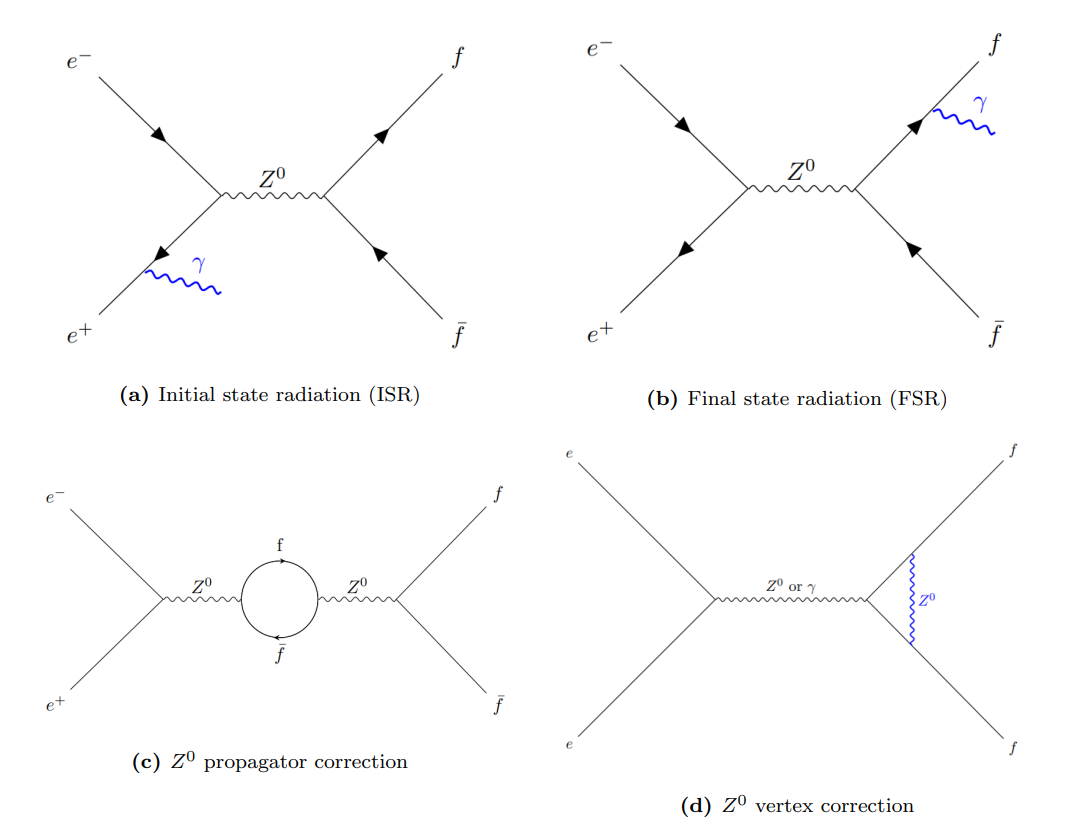
\includegraphics[width=\textwidth]{corrections}
\caption{Some radiative corrections}
\end{figure}
\end{minipage}\hspace{1em}
\begin{minipage}{0.45\textwidth}
To test out predictions of the Standard Model at high precision, need to account for higher order processes \footnotemark{}:
\begin{itemize}
\item \textbf{ISR:} radiation of photons in the initial state $\rightarrow$ decreases $\sqrt{s}$ and affects $Z^{0}$ peak parameters
\item \textbf{FSR:} radiation of photons or gluons in final state $\rightarrow$ partial widths increase
\item \textbf{Electroweak corrections:} Virtual processes like loops in $Z^{0}$ propagator and vertex corrections
\end{itemize}
\end{minipage}\hfill
\footcitetext{Zedometry}
\end{frame}
\subsubsection{Breit Wigner Distribution}
\begin{frame}
\frametitle{Breit Wigner Distribution}
\begin{itemize}
\item Contribution of $Z^{0}$ boson exchange propagator to the matrix element:
\vspace{0.5em}
$\mathcal{M}_{Z^{0}}\propto \dfrac{g_{Z^{0}}^{2}}{q^{2}-m_{Z^{0}}^{2}}=\dfrac{g_{Z^{0}}^{2}}{s-m_{Z^{0}}^{2}}$
\item Around the $Z^{0}$ resonance ($\sqrt{s}\sim  m_{Z^{0}}$), propagator diverges
\item Correction $\rightarrow$ modify propagator for a decaying state
\item For unstable particle having decay rate $\Gamma$, wavefunction modified to:
\vspace{0.5em}
$\psi\propto e^{-imt}\rightarrow e^{-imt}e^{-\Gamma t/2}$
\item Equivalent to introducing an additional imaginary term in the mass:
\vspace{0.5em}
$m\rightarrow m-i\dfrac{\Gamma}{2}$
\item $Z^{0}$ propagator then changes to:
\vspace{0.5em}
$\dfrac{1}{s-m_{Z^{0}}^{2}}\rightarrow \dfrac{1}{s-{\left(m_{Z^{0}}-i\Gamma_{Z^{0}}/2\right)}^{2}}$
\end{itemize}
\end{frame}

\begin{frame}
\frametitle{Breit Wigner Distribution}
\begin{minipage}{0.5\textwidth}
\begin{itemize}
\item Complete form of cross section in process $e^{+}e^{-}\rightarrow Z^{0}\rightarrow f\bar{f}$ is:
\vspace{0.5em}
$\sigma_f (s) = \frac{12\pi}{M_Z^2} \frac{s \Gamma_e \Gamma_f}{(s-M_Z^2)^2 + \left(\frac{s\Gamma_Z}{M_Z}\right)^2} (\hbar^2 c^2)$
\item \textbf{Breit-Wigner distribution:} Probability distribution that characterizes this dependence of cross section on centre of mass energy 
\item Various physical parameters can be extracted by fitting this theoretical distribution to the observed data
\end{itemize}
\end{minipage}\hspace{0.5em}
\begin{minipage}{0.45\textwidth}
\begin{figure}
\centering
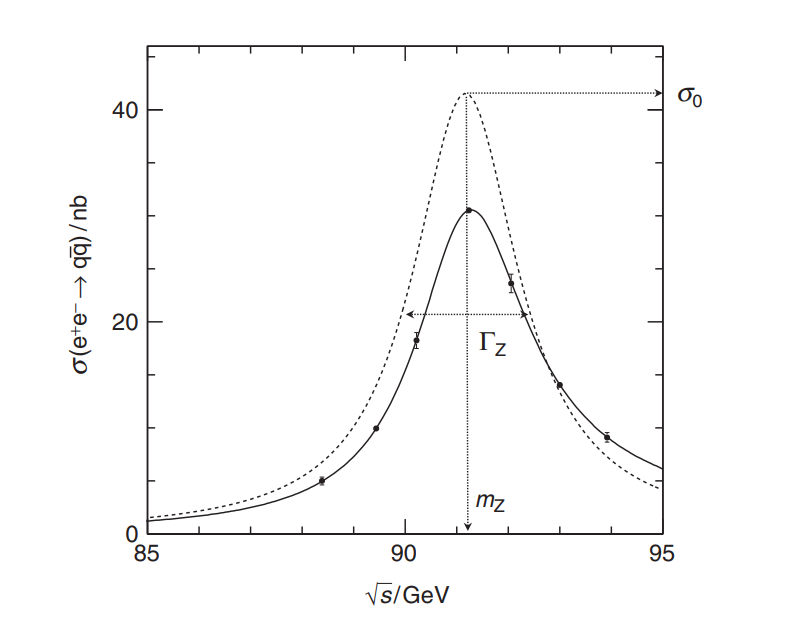
\includegraphics[width=\textwidth]{BWdist}
\caption{Breit Wigner distribution of the cross section for $e^{+}e^{-}\rightarrow q\bar{q}$ process \footnotemark{}}
\end{figure}
\end{minipage}
\footcitetext{thomson_2013}
\end{frame}

\subsubsection{LEP Experiment and OPAL Detector}
\begin{frame}
\frametitle{The LEP Experiment}
\begin{itemize}
\item LEP built at CERN; started operating in 1989
\item One of the major goals: make high precision measurements of $Z^{0}$ boson properties
\item Produced $e^{+}e^{-}$ collisions at $\sqrt{s}$ close to $Z^{0}$ resonance 
\item Recorded about 17 million $e^{+}e^{-}\rightarrow Z^{0}$ events (1989-95) \footnotemark{}
\item Collisions at four different points in the circular collider $\rightarrow$ four detectors:
\begin{itemize}
\item ALEPH (Apparatus for LEP PHysics)
\item DELPHI (DEtector with Lepton, Photon and Hadron Identification)
\item L3 (Third LEP experiment)
\item OPAL (Omni-Purpose Apparatus for LEP)
\end{itemize}
\end{itemize}
\footcitetext{thomson_2013}
\end{frame}

\begin{frame}
\frametitle{OPAL Detector and its Components}
\begin{minipage}{0.5\textwidth}
Starting from origin, as $e^{+}e^{-}$ collision products fly outwards, various detector components are encountered. These are discussed here in brief:
\begin{itemize}
\item \textbf{Vertex detector:} 
\begin{itemize}
\item Surrounds the central beam pipe
\item Key role: locating vertices of short-lived decay products
\item Improves momentum resolution
\end{itemize}
\item \textbf{Jet chamber:}
\begin{itemize}
\item Has good spatial and track resolution
\item Records events associated with jets
\item Also determines $dE/dx$ of charged particles
\end{itemize} 
\end{itemize}
\end{minipage}\hspace{0.5em}
\begin{minipage}{0.45\textwidth}
\begin{figure}
\centering
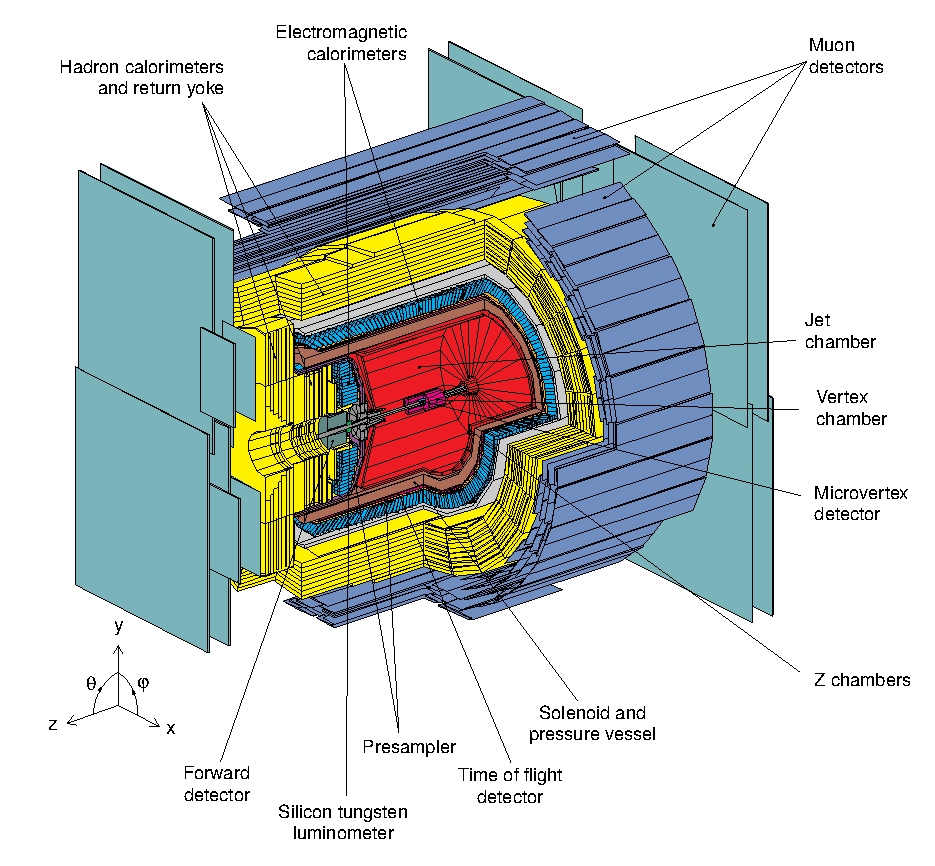
\includegraphics[width=\textwidth]{OPAL1}
\caption{Cross sectional view of the OPAL detector \footnotemark{}}
\end{figure}
\end{minipage}
\footcitetext{OPAL}
\end{frame}

\begin{frame}
\frametitle{OPAL Detector and its Components}
\begin{itemize}
\item \textbf{$\mathbf{z}$ chambers:}
\begin{itemize}
\item Locates $z$ coordinates of decay particles
\item Helpful in improving the resolutions of the polar angle
\end{itemize}
\item \textbf{Solenoid:}
\begin{itemize}
\item Surrounds central detector
\item Generates a uniform magnetic field of 0.435 T along beam dirn.
\item $\vec{B}$ field $\rightarrow$ particles have helical path $\rightarrow$ momenta can be measured
\end{itemize}
\item \textbf{Time of flight (TOF) system:}
\item \textbf{ECAL:}
\item \textbf{HCAL:}
\item \textbf{Muon detector:}
\end{itemize}
\end{frame}
\section*{References}
\begin{frame}
\frametitle{References}
\printbibliography
\end{frame}
\end{document}